\documentclass[sigconf]{acmart}

\usepackage{booktabs} % For formal tables

% Copyright
%\setcopyright{none}
\setcopyright{acmcopyright}
%\setcopyright{acmlicensed}
%\setcopyright{rightsretained}
%\setcopyright{usgov}
%\setcopyright{usgovmixed}
%\setcopyright{cagov}
%\setcopyright{cagovmixed}


% DOI
\acmDOI{xx.xxx/xxx_x}

% ISBN
\acmISBN{978-1-4503-6866-7/20/03}

%Conference
\acmConference[SAC'20]{ACM SAC Conference}{March 30-April 3, 2020}{Brno, Czech Republic} 
\acmYear{2020}
\copyrightyear{2020}


\acmArticle{4}
\acmPrice{15.00}

% These commands are optional
%\acmBooktitle{Transactions of the ACM Woodstock conference}
%\editor{Jennifer B. Sartor}
%\editor{Theo D'Hondt}
%\editor{Wolfgang De Meuter}


\begin{document}
% title should have "Student Research Abstract"
% title should have "Student Research Abstract"
% title should have "Student Research Abstract"
\title{Student Research Abstract: Title of Your Abstract}
% title should have "Student Research Abstract"
% title should have "Student Research Abstract"
% title should have "Student Research Abstract"

%\titlenote{Produces the permission block, and
%  copyright information}
%\subtitle{Extended Abstract}
%\subtitlenote{The full version of the author's guide is available as
%  \texttt{acmart.pdf} document}


\author{Ben Trovato}
%\authornote{Dr.~Trovato insisted his name be first.}
\orcid{1234-5678-9012}
\affiliation{%
  \institution{Institute for Clarity in Documentation}
  \streetaddress{P.O. Box 1212}
  \city{Dublin} 
  \state{Ohio} 
  \postcode{43017-6221}
}
\email{trovato@corporation.com}

% The default list of authors is too long for headers}
\renewcommand{\shortauthors}{B. Trovato et al.}

\begin{abstract}
This paper provides a sample of a \LaTeX\ document which conforms,
somewhat loosely, to the formatting guidelines for
ACM SIG Proceedings.
\end{abstract}

%
% The code below should be generated by the tool at
% http://dl.acm.org/ccs.cfm
% Please copy and paste the code instead of the example below. 
%
\begin{CCSXML}
<ccs2012>
 <concept>
  <concept_id>10010520.10010553.10010562</concept_id>
  <concept_desc>Computer systems organization~Embedded systems</concept_desc>
  <concept_significance>500</concept_significance>
 </concept>
 <concept>
  <concept_id>10010520.10010575.10010755</concept_id>
  <concept_desc>Computer systems organization~Redundancy</concept_desc>
  <concept_significance>300</concept_significance>
 </concept>
 <concept>
  <concept_id>10010520.10010553.10010554</concept_id>
  <concept_desc>Computer systems organization~Robotics</concept_desc>
  <concept_significance>100</concept_significance>
 </concept>
 <concept>
  <concept_id>10003033.10003083.10003095</concept_id>
  <concept_desc>Networks~Network reliability</concept_desc>
  <concept_significance>100</concept_significance>
 </concept>
</ccs2012>  
\end{CCSXML}

\ccsdesc[500]{Computer systems organization~Embedded systems}
\ccsdesc[300]{Computer systems organization~Redundancy}
\ccsdesc{Computer systems organization~Robotics}
\ccsdesc[100]{Networks~Network reliability}


\keywords{ACM proceedings, \LaTeX, text tagging}


\maketitle

\section*{PROBLEM AND MOTIVATION}
The student research abstract (SRA) will be published both in the
printed proceedings of ACM SAC and later in ACM digital
library. The proceedings are the records of the conference. To do
this, we ask that student authors follow some simple guidelines. In
essence, we ask you to make your research abstract look exactly
like this document. The easiest way to do this is simply to
download a template from the website of ACM SAC, and replace
the content with your own material, which includes \emph{the innovation
behind the proposed research idea and the applicability of
anticipated results to real-world problems; the problem being
investigated; the proposed solution and research methodology;
and sample preliminary results of the work.}

\section*{BACKGROUND AND RELATED WORK}
All material on each page should fit within a rectangle of 18 x
23.5 cm (7" x 9.25"), centered on the page, beginning 2.54 cm
(1") from the top of the page and ending with 2.54 cm (1") from
the bottom. The right and left margins should be 1.9 cm (.75").
The text should be in two 8.45 cm (3.33") columns with a .83 cm
(.33") gutter.

\section*{APPROACH AND UNIQUENESS}
\subsection*{Normal or Body Text}
Please use a 9-point Times Roman font, or other Roman font with
serifs, as close as possible in appearance to Times Roman in
which these guidelines have been set. The goal is to have a 9-
point text, as you see here. Please use sans-serif or nonproportional
fonts only for special purposes, such as
distinguishing source code text. If Times Roman is not available,
try the font named Computer Modern Roman. On a Macintosh,
use the font named Times. Right margins should be justified, not
ragged.

\subsection*{Title and Authors}
The title (Helvetica 18-point bold), authors' names (Helvetica 12-
point) and affiliations (Helvetica 10-point) run across the full
width of the page - one column wide. The title should start with
"Student Research Abstract: ". We also recommend e-mail
address (Helvetica 12-point). See the top of this page for example.

\subsection*{Subsequent Pages}
For pages other than the first page, start at the top of the page, and
continue in double-column format. The two columns on the last
page should be as close to equal length as possible.

\begin{table}[h]
\caption{Table captions should be placed above the table}
\begin{tabular}{|c|c|c|c|}
\hline
Graphics & Top & In-between & Bottom \\
\hline
Tables & End & Last & First \\
\hline
Figures & Good & Similar & Very well \\
\hline
\end{tabular}
\end{table}

\begin{figure}
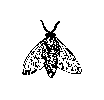
\includegraphics{fly}
\caption{A sample black and white graphic.}
\end{figure}

\begin{figure}
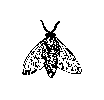
\includegraphics[height=1in, width=1in]{fly}
\caption{A sample black and white graphic
that has been resized with the \texttt{includegraphics} command.}
\end{figure}

\subsection*{References and Citations}
Footnotes should be Times New Roman 9-point, and justified to
the full width of the column.

Use the standard Communications of the ACM format for
references - that is, a numbered list at the end of the article,
ordered alphabetically by first author, and referenced by numbers
in brackets \cite{Smith10}. See the examples of citations at the end of this
document. Within this template file, use the style named
references for the text of your citation.

The references are also in 9 pt., but that section (see Section 7) is
ragged right. References should be published materials accessible
to the public. Internal technical reports may be cited only if they
are easily accessible (i.e. you can give the address to obtain the
report within your citation) and may be obtained by any reader.
Proprietary information may not be cited. Private communications
should be acknowledged, not referenced (e.g., "[Robertson,
personal communication]").

A couple of citations with DOIs: \cite{2004:ITE:1009386.1010128,
  Kirschmer:2010:AEI:1958016.1958018}. 

Online citations: \cite{TUGInstmem, Thornburg01, CTANacmart}.  

\subsection*{Page Numbering, Headers and Footers}
Do not include headers, footers or page numbers in your
submission. These will be added when the publications are
assembled.

\section*{RESULTS AND CONTRIBUTIONS}
Place Tables/Figures/Images in text as close to the reference as
possible (see Figure 1). It may extend across both columns to a
maximum width of 17.78 cm (7").

Captions should be Times New Roman 9-point bold. They should
be numbered (e.g., "Table 1" or "Figure 2"), please note that the
word for Table and Figure are spelled out. Figure's captions should be centered beneath the image or picture, and Table captions should be centered above the table body.

\bibliographystyle{ACM-Reference-Format}
\bibliography{sample-bibliography} 

\end{document}
